%  Prerequisites
\chapter{State of the Art}
This chapter provides an overview of the concepts and technologies which are important in the field of my current work. First in Section \ref{lab:background} we define domain-specific terms. In Section \ref{lab:systems}, we describe the systems, which will be used for this thesis.

\section{Background} \label{lab:background}

This section gives a brief introduction to the concepts, which are relevant to the implementation part of this thesis.

\subsection{Social Bots and Chatbots}
Bots in general are an interfaces, which provide automated services to end-users.
In contrast to normal computer programs, bots use the services, which were designed for human users, such as browsing webpages and issuing API calls.
Bots, which are deployed in social media, are called social bots.
The definition of a social bot is provided by \cite{FVD*16b}:
\begin{quote}
	``A social bot is a computer algorithm that automatically produces content and interacts with humans on social media, [...]''
\end{quote}

Social bots are getting more and more popular in Human-Computer Interactin (HCI), by integrating automation into daily lives of people \cite{BFPN17}. Users can interact with a social bot through a dedicated channel, such as the chat functionality of a social network.
Social bots, which use chats to interact with users are called chatbots, or conversational bots \cite{WWX*16}.
Chatbots have recently become very popular in the context of customer care \cite{CHW*17,FVD*16b}, where they act as virtual assistants, which can answer simple questions \cite{CaWh14} or perform predefined tasks.
They thereby assist companies in customer service as they are more economical and the staff can concentrate on less mundane tasks.

Chatbots can be classified into chit-chat chatbots, or task-oriented bots.
A chit-chat bot engages users into interesting conversations.

We can distinguish between retrieval based chatbots and generic chatbots \cite{NLKl19,WWX*16}.
Retrieval based bots are focussed on getting specific tasks done and focus less on engaging in a coherent conversation.

Retrieval based chatbots measure the similarity of user queries to candidate responses and run the task that is defined for that response.
They do this by using natural language processing techniques.
Generic chatbots on the other hand also produce generic responses.
An advantage of the generic chatbots is that they provide a better user experience as users can interact more naturally with them than with retrieval based chatbots.

Chatbots provide a better user experience \cite{CHW*17}, because the user is not required to memorize commands in order to get the desired results.
This means that even non-trained users can use such chatbots.
From such a standpoint, it becomes clear why such chatbots are desirable as assistants, as they provide a familiar environment for users to interact with.

\subsubsection{Natural Language Understanding}
Natural Language Understanding (NLU) is a branch of Artificial Intelligence (AI), which tries to make computer programs understand the semantics of human language.
It does this by transforming a block of input text into a data structure that is programmer-friendly but still describes the original meaning of the text \cite{CWB*11}.

Most NLU algorithms these days only look at the syntacticts of words, which relies on statistical features, such as word occurence frequency \cite{CaWh14}.
However humans take far more information into consideration, as the reading of a word triggers a whole bunch of related concepts and experiences which are combined to give the understanding of a text.

Computers try to close this knowledge gap with computational models, which emulate human cognitive processing.
By evaluating the results of those models for a given input, researchers can incrementally improve the accuracy of the model \cite{CaWh14}


\subsection{Communities of Practice}
Humans naturally gather in groups, which share a particular property, such as a common goal.
Members of this group are distinguishable from people outside of this group by that particular property.
Such groups are called communities.

Communities of Practice (CoP) are groups of people who share a concern or a passion for something they do and who interact regularly to learn how to do it better \cite{Weng98}.
Such CoPs are caracterized by a small number of members.
The advantage of CoPs is that they enhance learning and transferring knowledge inside the community.
In contrast to traditional knowledge systems, where the learner digests a static body of information, the transfer of knowledge is a dynamic social process, where an individual volontarily shares knowledge in the community \cite{AMMi15,Kern08}.

The use of communities improves the qualitity of activities and makes the learning process easier\cite{SaAr05} and faster\cite{CuZe05}.
Members of CoPs do not have to belong to the same organization, but rather participate in common work through the use of social networks\cite{CuZe05}.

\subsection{Measurement of Success}
In order to justify their existence, communities have to constantly be aware of their successes and failures in order to improve their work and adjust to current needs.
A general model for success does not exist, as communities are very diverse, dynamic and informal structures with permeable boundaries.
The members of the community thus can be active participators in the community success modeling, as the success factors are relevant to the practice of the community members \cite{RKJa15}.

In order to cope with dynamic changes, the community must continiously adjust success factors of the success model to satisfy current needs. Success factors can be internal aspects, like project duration, cost and qualitity, as well as external aspects, like customer satisfaction \cite{AgRa06}.

It is important to note, that a project can be evaluated from different perspectives \cite{RKJa15}, e.g. the developers, the customers or the end-users.
In each of these perspectives, each dimension of success can be more, or less, important.
DeLone and McLean \cite{DeMc92} base their model on six different interdependant measures:
\begin{itemize}
	\item System Qualitity: metrics that describe the technical specifations of the system, such as service response time and scalability.
	\item Information Quality: metrics about content qualitity,such as understandability and conciseness.
	\item Use: Metrics about how a system is used, such as the regularity of use by a certain user or for the whole community.
	\item User Satisfaction: includes metrics which measure user experience and is thereby largely subjective.
	\item Individual Impact: metrics about how a user adapts to the system over time, such as task performance and user learning
	\item Organizational (Community) Impact: metrics about how the system influences the organization (or community) over time
\end{itemize}
\begin{figure}[!h]
	\centering
	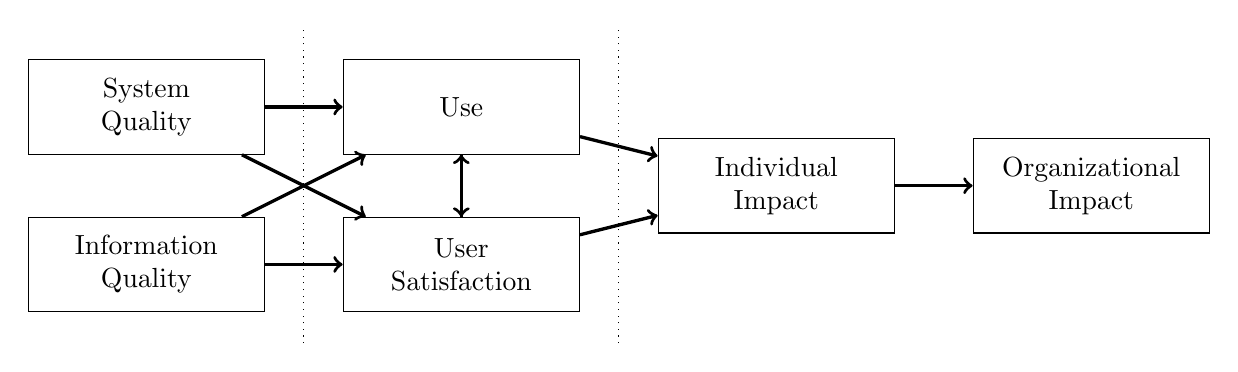
\begin{tikzpicture}[node distance=3.0cm and 6.0cm]
		\node[draw, align=center, minimum width=3cm, minimum height=1.2cm] at (0,2) (SysQ) {System\\ Quality};
		\node[draw, align=center, minimum width=3cm, minimum height=1.2cm] at (0,0) (InfoQ) {Information\\ Quality};
		\node[draw, align=center, minimum width=3cm, minimum height=1.2cm] at (4,2) (Use) {Use};
		\node[draw, align=center, minimum width=3cm, minimum height=1.2cm] at (4,0) (UserSat) {User\\ Satisfaction};
		\node[draw, align=center, minimum width=3cm, minimum height=1.2cm] at (8,1) (Indivi) {Individual\\ Impact};
		\node[draw, align=center, minimum width=3cm, minimum height=1.2cm] at (12,1) (Orga) {Organizational\\ Impact};
		\draw [->, very thick] (InfoQ) -- (Use);
		\draw [->, very thick] (InfoQ) -- (UserSat);
		\draw [->, very thick] (SysQ) -- (Use);
		\draw [->, very thick] (SysQ) -- (UserSat);
		\draw [->, very thick] (Use) -- (Indivi);
		\draw [->, very thick] (UserSat) -- (Indivi);
		\draw [->, very thick] (Use) -- (UserSat);
		\draw [->, very thick] (UserSat) -- (Use);
		\draw [->, very thick] (Indivi) -- (Orga);
		\draw[dotted] (2,-1) -- (2,3);
		\draw[dotted] (6,-1) -- (6,3);
	\end{tikzpicture}
	\caption{Community Information Systems Success Model by DeLone and McLean~\cite{DeMc92}}
	\label{CISModel}
\end{figure}
In order to collect data for the metrics, one should follow the principle \cite{RKJa15}:
\begin{quotation}
	``observe, where possible; only survey,	where inevitable''
\end{quotation}

\subsection{Mediabase}
Mediabase has been proposed to store Web 2.0 data in a dynamic way \cite{KlPe08}.
Mediabase uses graphs to model generated data.
The nodes in those graphs are called \emph{Actors} and represent either a \emph{ Medium}, an \emph{Artifact}, a \emph{Member}, or a \emph{Network}.
A \emph{ Medium} can be a blog or a wiki. 
The \emph{Artifact} would be an individual entry.
The \emph{Network} represents the community, in which the different \emph{Members} interact in.
\emph{Members} do not have to be human, but are assigned a specific role in the \emph{Network}.
\begin{figure}
	\centering
	\includegraphics*[width=12cm]{related_work/mediabase.png}
	\caption{Mediabase Overview \cite{Klam10e}}
\end{figure}
Furthermore, Mediabase includes \emph{Services}.
A Mediabase consists of a backend database, like DB2, or MySQL, crawler scripts and monitoring processes and a frontend for visualization of data  and user interaction.

This approach is favorable for the management of large scale-free dynamic social graphs.

\section{Systems} \label{lab:systems}
Creating a chatbot from scratch is a difficult challenge. Luckily, there are already publicly available frameworks, which can be used to create a variety of bots.

\subsection{Social Bot Framework}

The Social Bot Framework (SBF) is a Web-based model-driven near-realtime environment to develop chatbots \cite{NLKl19}. The model-driven development allows less experienced users to take part in the development, which is favorable for the creation of a chatbot inside a Community of Practice (CoP). The framework consists of a GUI to model the bot and define the actions, which it should perform, and a Social Bot Manager Service, which is used to deploy the bot.

\subsection{RASA}
Rasa is an open sourced framework for building chat- and voice-based bots. The goal of RASA is to bring current advances in machine-learning to end-users, such that they can create chatbots in a simple way \cite{BFPN17}. The RASA system is split into a component for natural language understanding (RASA NLU) and a dialogue management component (RASA Core).

RASA NLU is used to extract the intents of a user message with a text classification based on the fastText approach \cite{BFPN17}. fastText has a similar accuracy to conventional deep learning classifiers, but is much faster and therefore more easily scalable \cite{JGBM16}.

RASA Core consists of a \emph{Tracker}, a \emph{Policy} and a set of \emph{Actions} \cite{BFPN17}. The Tracker manages the current state of the conversation. It gets an intent as an input and forwards it the Policy, which selects the next action, given the current state of the conversation and a predefined list of actions for each intent. The Action triggers the Tracker to recalculate the new state and might also send a reply to the user.

The system is built in a modularized way and each service provides HTTP APIs \cite{BFPN17}, which makes it possible to use the NLU component independantly of the rest of the framework. This makes it easy to integrate it into an existing system \cite{RaKe19}.

\subsection{MobSOS}
The MobSOS framework is a tool, which assists online communities in monitoring and evaluating services. The MobSOS success model extends the classical D\&M IS success model by adding feature aspects which were not covered initially, such as Qualitity of Service and mobility \cite{Renz08}.
The MobSOS Success Modeling concept is described as an iterative process.

The MobSOS Continuous Community Analytics (CCA) system extends the MobSOS framework by providing visualizations of MobSOS data and the ability to add more databases, which can be used for success modeling.

\subsection{las2peer}
las2peer is a disributed platform, which allows users to easily deploy their HTTP services. Each service is a node in the network and many nodes can form a peer-to-peer seed network, which communicate through standard protocols. Data storage and communications are encrypted, adding an extra layer of security to las2peer services. This allows even small communities to securely design and deploy las2peer services.

The las2peer platform contains the MobSOS framework, but not the CCA.

\subsection{Google Charts API}
Google Charts API\footnotemark is an API that provides visualizations for database data. The data, which should be visulaized needs to be wrapped inside a Javascript class called \texttt{DataTable}, which represents a two-dimensional table with rows and columns, where each column has a datatype.
A new column can be added using the \texttt{DataTable.addColumn} function, which takes the type and name as input. An example can be seen in Listing \ref{lst:gglCharts} from the Google Charts API documentation\footnotemark[\value{footnote}].

\begin{lstlisting}[caption=Example use of the DataTable class,captionpos=b,label={lst:gglCharts}]
var data = new google.visualization.DataTable();
data.addColumn('string', 'Topping');
data.addColumn('number', 'Slices');
data.addRows([
	['Mushrooms', 3],
	['Onions', 1],
	['Olives', 1], 
	['Zucchini', 1],
	['Pepperoni', 2]
]);
\end{lstlisting}


The visualizations are rendered as SVGs in the browser, but can be the PNG file can be accessed by maken an http call with the \texttt{getImageURI} as image URI parameter.

\footnotetext{\href{https://developers.google.com/chart}{Google Charts API}}